
\subsection{\textbf{Etat de l'art des modeles de d'etection de têtes}}

La détection des têtes est un sujet fondamental en vision par ordinateur, notamment pour des applications variées telles que la surveillance, l'analyse de foules, et les interactions homme-machine. Ce probl`eme est souvent abordé avec des techniques similaires à celles de la détection d'objets, en particulier les approches basées sur l'apprentissage profond.

\subsubsection{\textbf{Modèles basés sur les Réseaux de Neurones Convolutifs (CNNs)}}
Les CNNs sont les architectures les plus populaires pour la détection d'objets en raison de leur capacité à extraire des caractéristiques discriminantes \cite{lecun1998gradient}. Les architectures telles que Faster R-CNN \cite{ren2015faster}, SSD \cite{liu2016ssd} et RetinaNet \cite{lin2017focal} ont été adaptées pour la détection des têtes en raison de leur capacité à gérer des objets de différentes tailles.

\subsubsection{\textbf{Modèles basés sur YOLO}}
YOLO (You Only Look Once) est une famille de modèles de détection d'objets qui allie vitesse et précision \cite{redmon2016you}. Depuis YOLOv1 jusqu'à YOLOv11, les améliorations successives ont permis d'obtenir des performances toujours plus optimales en termes de précision et d'efficacité \cite{bochkovskiy2020yolov4, jocher2023ultralytics}. YOLO est particulièrement adapté à la détection en temps réel, ce qui le rend pertinent pour des applications de surveillance et de comptage de personnes \cite{ge2019efficient, lian2021locating}. 
Récemment, YOLOv12 \cite{tian2025yolov12attentioncentricrealtimeobject} a introduit une architecture centrée sur les mécanismes d'attention tout en maintenant une vitesse d'inférence comparable aux mod`eles CNN classiques. Cette approche permet d'améliorer la précision de la détection tout en conservant des performances adaptées aux besoins des applications en temps réel.
\subsection{Datasets}

Il existe plusieurs datasets pour la détectiond des têtes et avec l'utilisation grandissante des cameras comme moyens de surveillance, ils se sont multipliés et sont de plus en plus gros. On dispose donc de beaucoup de matériel pour notre entrainement et évaluation, certains articles \cite{state_of_the_art_datasets} proposent des benchmarks pour les datasets les plus utilisés.

Pour notre utilisation, nous cherchons des datasets avec un nombre de personne supérieur à 100, car nous souhaitons nous intérresser spécifiquement aux foules denses. Pour cela nous avons sélectionnés les datasets JHU-Crowd++ \cite{sindagi2020jhu-crowd++} (le seul utilisé dans ce projet en réalité) qui présente 4372 avec en moyenne 346 personnes et jusque 25,791.
Nous avons selectionné 2 autres datasets semblables que nous n'avons pas utilisé dans ce projet, le NWPU-Crowd \cite{gao2020nwpu} avec 5,109 images d'en moyenne 418 personnes, et le UCF-QNRF \cite{idress2018ucfqnrf} avec 1,535 images d'en moyenne 815 personnes.

\subsection{Finetuning}

ILANN BLABLABLA

\subsection{Résultats qualitatifs}

Comme vous pouvez le voir sur l'exemple Figure \ref{fig:heads-detection}, la détection des têtes est plutôt bonne, lorsque l'on est dans les champs proches et/ou que l'on voit bien l'entièreté de la tête.

Cependant le modèle atteint ses limites lorsqu'il y a beaucoup de têtes sur l'image, ou que celles-ci sont partiellement caché ou en mauvaise résolution (car trop loin)
.
\begin{figure}[h!]
    \centering
    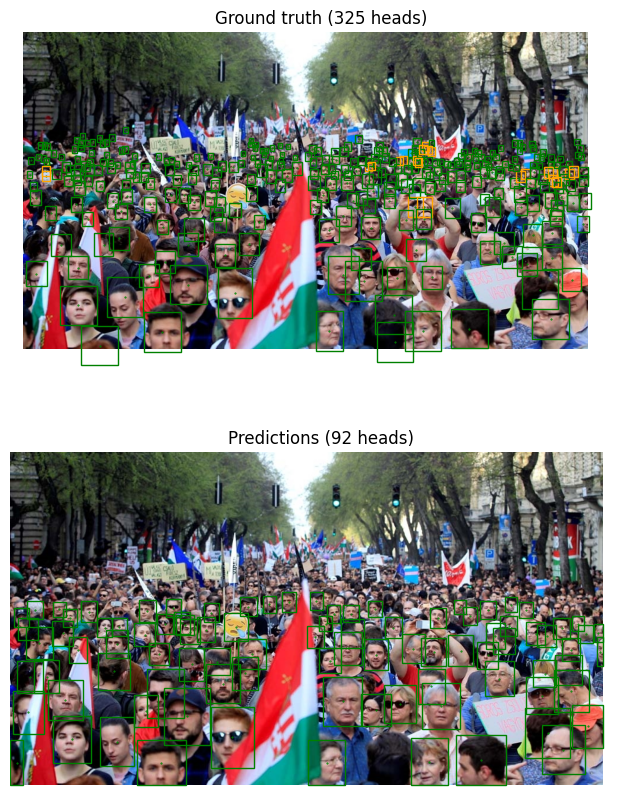
\includegraphics[width=0.45\textwidth]{images/heads_detection.png}
    \caption{Résultats qualitatif de la détection des têtes.}
    \label{fig:heads-detection}
\end{figure}